\documentclass[oneside]{book}
%---------------PREAMBLE------------%
\usepackage{geometry}
\geometry{a4paper, margin = 1.0in}
\usepackage[dvipsnames]{xcolor}
\usepackage{graphicx}
\usepackage{mathtools}
\usepackage{amsfonts,amsthm,esint,mathrsfs}
\usepackage[font={scriptsize,it}]{caption}
\usepackage{float}
\usepackage{multicol}
\usepackage[font={scriptsize}]{subcaption}
\usepackage{pgfplots,tikz}
\usepgfplotslibrary{groupplots}
\usetikzlibrary{calc,patterns,angles,quotes,arrows,arrows.meta,shapes,shapes.geometric,cd,hobby,positioning,decorations.markings}
\pgfplotsset{compat=1.9}
\usepackage{hyperref}
\hypersetup{colorlinks=true,linkcolor=blue,filecolor=magenta,urlcolor=Cerulean,citecolor=SkyBlue}
\graphicspath{{images/}}
%-------------New Commands----------%
\renewcommand\thesubfigure{\arabic{chapter}.\arabic{figure}.\arabic{subfigure}}
\newcommand{\MarkRightAngle}[4][.3cm]% #1=size (optional), #2-#4 three points: \angle #2#3#4
{\coordinate (tempa) at ($(#3)!#1!(#2)$);
 \coordinate (tempb) at ($(#3)!#1!(#4)$);
 \coordinate (tempc) at ($(tempa)!0.5!(tempb)$);%midpoint
 \draw (tempa) -- ($(#3)!2!(tempc)$) -- (tempb);}
%-------------Tikz Preset-----------%
\pgfdeclareradialshading{myring}{\pgfpointorigin}{%
    color(0cm)=(transparent!0);
    color(5mm)=(pgftransparent!50);
    color(1cm)=(pgftransparent!100)%
}
\pgfdeclarefading{ringo}{\pgfuseshading{myring}}
\pgfdeclareradialshading{red normal}{\pgfqpoint{0bp}{0bp}}{%
    color(0bp)=(white);
    color(10bp)=(red!90!black);
    color(20bp)=(black!75!red);
    color(30bp)=(black);
    color(100bp)=(black)%
}
\pgfdeclareradialshading{red distorted}{\pgfqpoint{10bp}{10bp}}{%
    color(0bp)=(white);
    color(10bp)=(red!90!black);
    color(20bp)=(black!75!red);
    color(30bp)=(black)%
}
\pgfdeclareradialshading{blue normal}{\pgfqpoint{0bp}{0bp}}{%
    color(0bp)=(white);
    color(10bp)=(blue!90!black);
    color(20bp)=(black!75!blue);
    color(30bp)=(black);
    color(100bp)=(black)%
}
\pgfdeclareradialshading{blue distorted}{\pgfqpoint{10bp}{10bp}}{%
    color(0bp)=(white);
    color(10bp)=(blue!90!black);
    color(20bp)=(black!75!blue);
    color(30bp)=(black)%
}
\pgfdeclareradialshading{gray distorted}{\pgfqpoint{10bp}{10bp}}{%
    color(0bp)=(white);
    color(25bp)=(black!100!gray)%
}
\pgfdeclareradialshading{gray normal}{\pgfqpoint{0bp}{0bp}}{%
    color(0bp)=(white);
    color(25bp)=(black!100!gray)%
}
\title{Examples and Templates}
\author{Ryan Maguire}
\date{December 2017}
\begin{document}
\maketitle
\tableofcontents
\listoffigures
\section{Tikz Package}
\subsection{The Team Cassini Pipeline}
\begin{figure}[H]
    \centering
    \resizebox{!}{0.8\textheight}{
    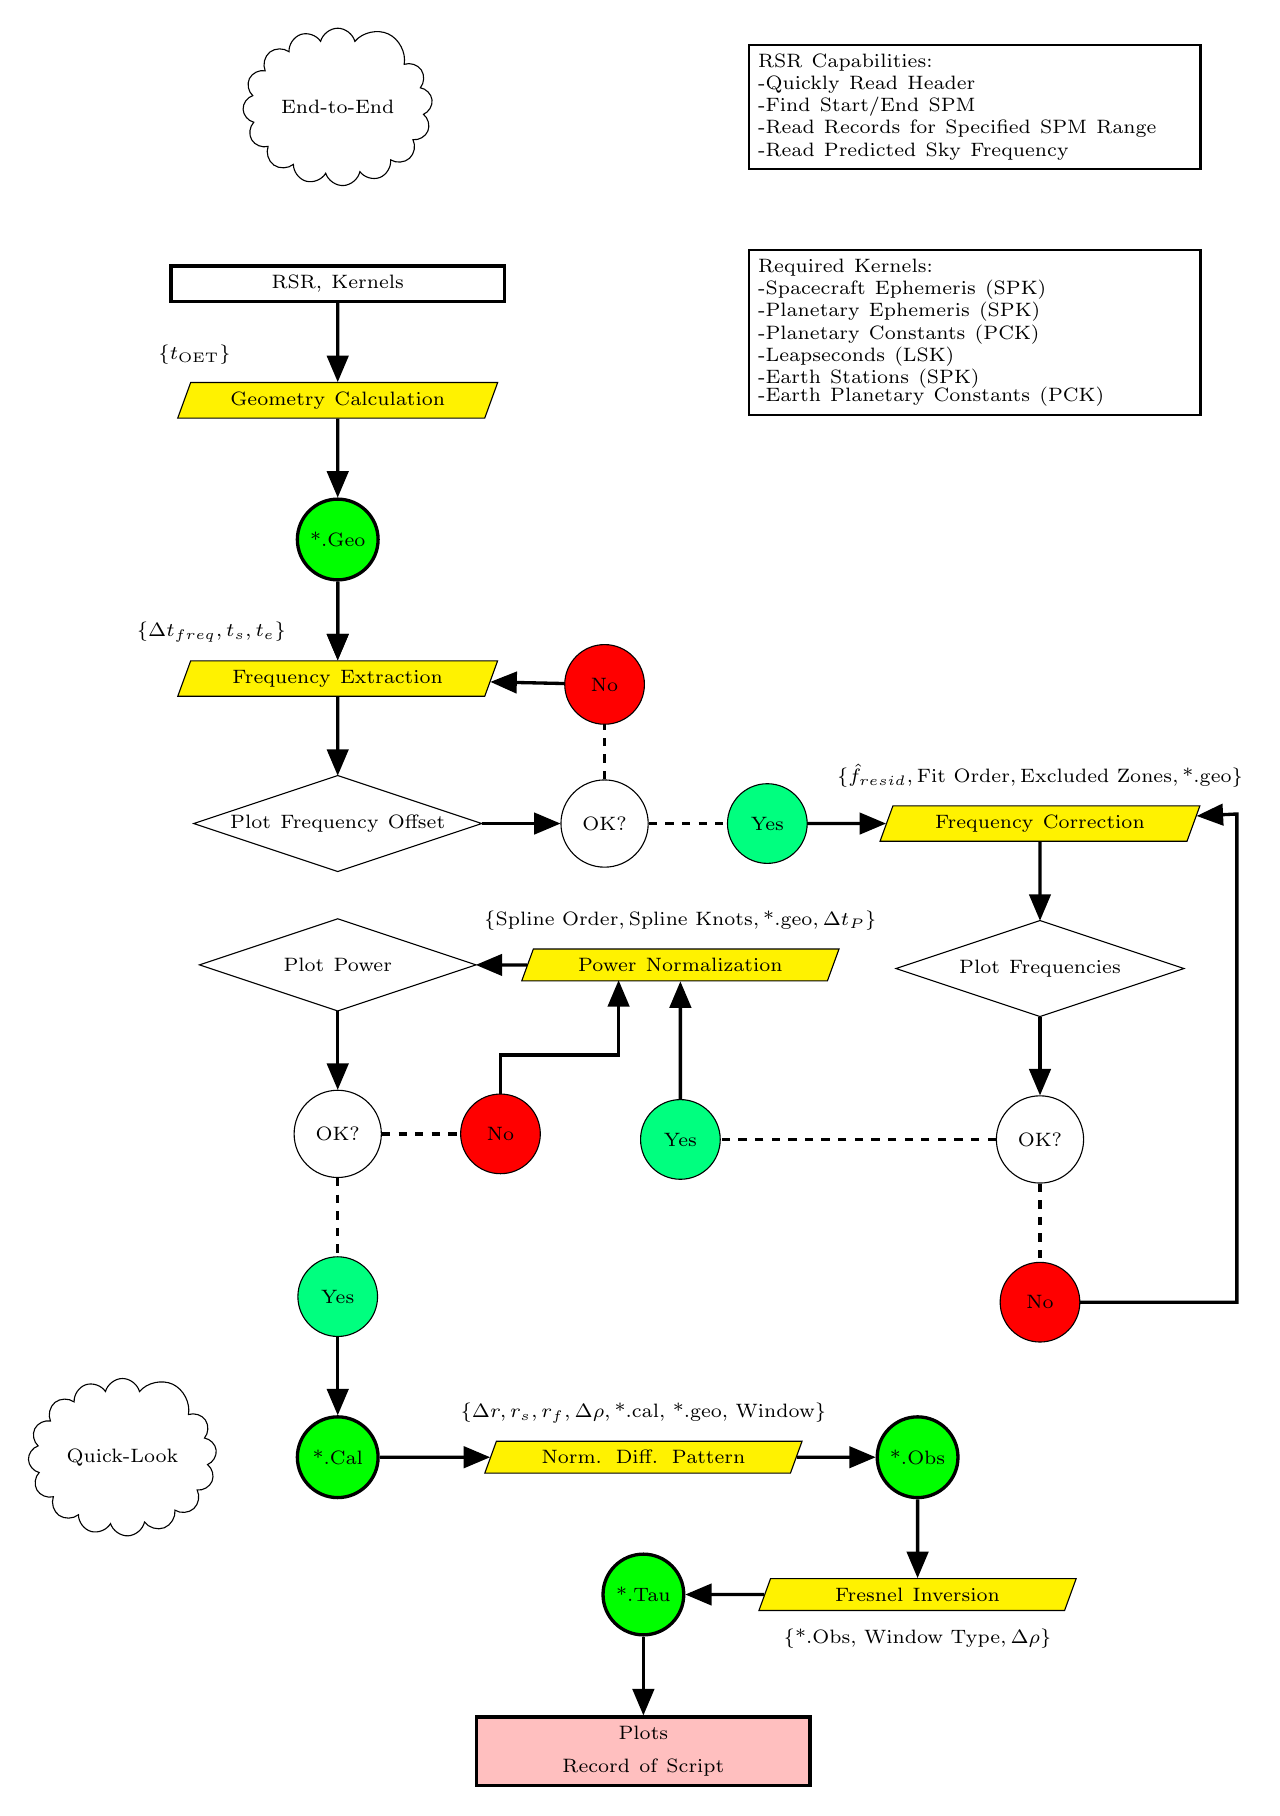
\begin{tikzpicture}
        %Nodes
        \begin{scope}[
            roundnode/.style={%
                circle, draw=black, very thick, text width=2em,
                text centered, fill=green%
            },
            squarednode/.style={%
                rectangle, text width=4em, text centered, draw=black,
                very thick, fill=SkyBlue%
            },
            bignode/.style={%
                rectangle, draw=black, very thick, text width=4cm,
                text centered%
            },
            every edge/.style={draw=black,very thick},
            bigbig/.style={rectangle, draw=black,thick,text width=5.5cm},
            every edge/.style={draw=black,very thick},
            trapanode/.style={%
                trapezium, trapezium left angle=70, trapezium right angle=-70,
                draw=black, fill=yellow, text width=3.5cm, text centered%
            },
            dianode/.style={%
                diamond, draw=black, text width = 3cm, text centered,
                aspect=3, inner sep = 0pt, outer sep = 0pt%
            },
            qnode/.style={circle,draw=black,text width = 8mm,text centered},
            nonode/.style={%
                circle, draw=black, fill=red,text width = 1cm, text centered,
                inner sep=0pt, outer sep=0pt%
            },
            yenode/.style={%
                circle, draw=black, fill=SpringGreen, text width=1cm,
                text centered, inner sep=0pt, outer sep=0pt%
            }
        ]
            \node[%
                cloud,cloud puffs=15.7, cloud ignores aspect,
                minimum height=2cm, align=center, draw,aspect=3%
            ] (0) {\scriptsize{End-to-End}};
            \node[bignode]   (1)  [below=of 0] {\scriptsize{RSR, Kernels}};
            \node[trapanode] (2)  [below=of 1] {\scriptsize{Geometry Calculation}};
            \node                 [above left=1mm and 10mm of 2]
                                    {\scriptsize{$\{t_{\textrm{OET}}\}$}};
            \node[roundnode] (3)  [below=of 2] {\scriptsize{*.Geo}};
            \node[trapanode] (4)  [below=of 3] {\scriptsize{Frequency Extraction}};
            \node                 [above left=1mm and 3mm of 4]
                                    {\scriptsize{$\{\Delta t_{freq},t_{s},t_{e}\}$}};
            \node[dianode]   (5)  [below=of 4]
                                    {\scriptsize{Plot Frequency Offset}};
            \node[qnode]     (6)  [right=of 5] {\scriptsize{OK?}};
            \node[nonode]    (6n) [above=7mm of 6] {\scriptsize{No}};
            \node[yenode]    (6y) [right=of 6] {\scriptsize{Yes}};
            \node[trapanode] (7)  [right=of 6y]
                                    {\scriptsize{Frequency Correction}};
            \node[dianode]   (7a) [below=of 7] {\scriptsize{Plot Frequencies}};
            \node[qnode]     (8)  [below=of 7a] {\scriptsize{OK?}};
            \node[nonode]    (8n) [below=of 8] {\scriptsize{No}};
            \node[yenode]    (8y) [left=3.5cm of 8] {\scriptsize{Yes}};
            \node[trapanode] (9)  [above=1.5cm of 8y]
                                    {\scriptsize{Power Normalization}};
            \node                 [above=1mm of 7] {%
                                        \scriptsize{$\{\hat{f}_{resid},
                                        \textrm{Fit Order},
                                        \textrm{Excluded Zones},
                                        \textrm{*.geo}\}$}
                                    };
            \node                 [above=1mm of 9] {%
                                        \scriptsize{%
                                            $\{\textrm{Spline Order},%
                                            \textrm{Spline Knots},%
                                            \textrm{*.geo},\Delta t_P\}$%
                                        }%
                                    };
            \node[dianode]   (10)  [below=6mm of 5]  {\scriptsize{Plot Power}};
            \node[qnode]     (11)  [below=of 10]     {\scriptsize{OK?}};
            \node[nonode]    (11n) [right=1cm of 11] {\scriptsize{No}};
            \node[yenode]    (11y) [below=1cm of 11] {\scriptsize{Yes}};
            \node[roundnode] (12)  [below=of 11y]    {\scriptsize{*.Cal}};
            \node[trapanode] (13)  [right=1.4cm of 12]
                                        {\scriptsize{Norm. Diff. Pattern}};
            \node                  [above=1mm of 13] {%
                                        \scriptsize{%
                                            $\{\Delta r, r_{s},r_{f},%
                                            \Delta \rho,%
                                            \textrm{*.cal, *.geo, Window}\}$%
                                        }%
                                    };
            \node[roundnode] (14)  [right=1cm of 13]  {\scriptsize{*.Obs}};
            \node[trapanode] (15)  [below=of 14] {\scriptsize{Fresnel Inversion}};
            \node[roundnode] (16)  [left =of 15] {\scriptsize{*.Tau}};
            \node[bignode,fill=pink]       (END) [below= of 16] {\scriptsize{Plots\\Record of Script}};
            \node                [below= 1mm of 15] {\scriptsize{$\{\textrm{*.Obs, Window Type},\Delta \rho\}$}};
            
            \node[cloud,cloud puffs=15.7, cloud ignores aspect, minimum height=2cm, align=center, draw] (QL) [left=of 12] {\scriptsize{Quick-Look}};
            %\node[rectangle, draw=black, very thick,text width=3cm,text centered,fill=yellow] (end) [below right = 0cm an%d 1cm of 9] {Plots and Record of Script};
            \node[bigbig]  (RSR) [right=4 cm of 0] {\scriptsize{RSR Capabilities:\\-Quickly Read Header\\-Find Start/End SPM\\-Read Records for Specified SPM Range\\-Read Predicted Sky Frequency\\}};
            \node[bigbig]  (Ker) [below=of RSR] {\scriptsize{Required Kernels:\\-Spacecraft Ephemeris (SPK)\\-Planetary Ephemeris (SPK)\\-Planetary Constants (PCK)\\-Leapseconds (LSK)\\-Earth Stations (SPK)\\\vspace{-0.7em}-Earth Planetary Constants (PCK)}};
        \end{scope}
        %Lines
        \begin{scope}[>={triangle 45},every edge/.style={draw=black,very thick}]
            \path[->] (1) edge (2);
            \path[->] (2) edge (3);
            \path[->] (3) edge (4);
            \path[->] (3) edge (4);
            \path[->] (4) edge (5);
            \path[->] (5) edge (6);
            \path[-,dashed] (6) edge (6n);
            \path[->] (6n) edge (4);
            \path[-,dashed] (6) edge (6y);
            \path[->] (6y) edge (7);
            \path[->] (7) edge (7a);
            \path[->] (7a) edge (8);
            \path[-,dashed] (8) edge (8n);
            \path[-,dashed] (8) edge (8y);
            \path[->] (8y) edge (9);
            \path[->] (9) edge (10);
            \path[->] (10) edge (11);
            \path[-,dashed] (11) edge (11n);
            \path[-,dashed] (11) edge (11y);
            \path[->] (11y) edge (12);
            \path[->] (12) edge (13);
            \path[->] (13) edge (14);
            \path[->] (14) edge (15);
            \path[->] (15) edge (16);
            \path[->] (16) edge (END);
            \draw[->,draw=black,very thick] (8n) -- ++(2.5cm,0) --++(0,6.2cm) -- (7);
            \draw[->,draw=black,very thick] (11n) -- ++(0,1cm) --++(1.5cm,0) --++ (0,0.95cm);
        \end{scope}
    \end{tikzpicture}}
    \caption[Data processing pipeline]{Data processing pipeline, with main steps in yellow, inputs in brackets above the main steps, files in bright green, intermediate plots as white rhombuses, test conditions as white circles, and test decisions as red and green circles. The End-to-End section begins at the very top, and the Quick-Look section begins near the bottom.}
    \label{fig:gjs_my_label}
\end{figure}
\subsection{Geometry}
\begin{figure}[H]
    \centering
    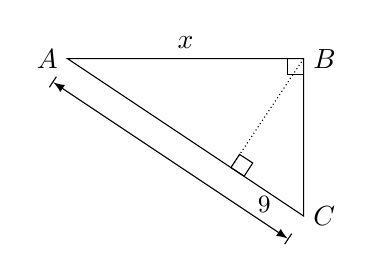
\begin{tikzpicture}
        \coordinate (A) at (0,0);
        \node at (A) [anchor = east] {$A$};
        \coordinate (B) at (3,0);
        \node at (B) [anchor = west] {$B$};
        \coordinate (C) at (3,-2);
        \node at (C) [anchor = west] {$C$};
        \draw (A)--(B)--(C)--cycle;
        \node at (1.5,0) [anchor = south] {$x$};
        \draw (B) rectangle +(-0.2,-0.2);
        \coordinate (D) at ($(A)!(B)!(C)$);
        \draw [densely dotted] (B)--(D);
        \draw [rotate = -33] (D) rectangle +(0.2,0.2);
        \node at (2.5,-1.85) {\small 9};
        \coordinate (D) at ($(A)+(-123:0.35)$);
        \coordinate (E) at ($(C)+(-123:0.35)$);
        \draw [|<->|, > = latex] (D) -- (E);
    \end{tikzpicture}
    \caption{Right Angle Triangle!}
    \label{fig:Triangle}
\end{figure}
\subsection{Group Plots}
\begin{figure}[H]
    \centering
    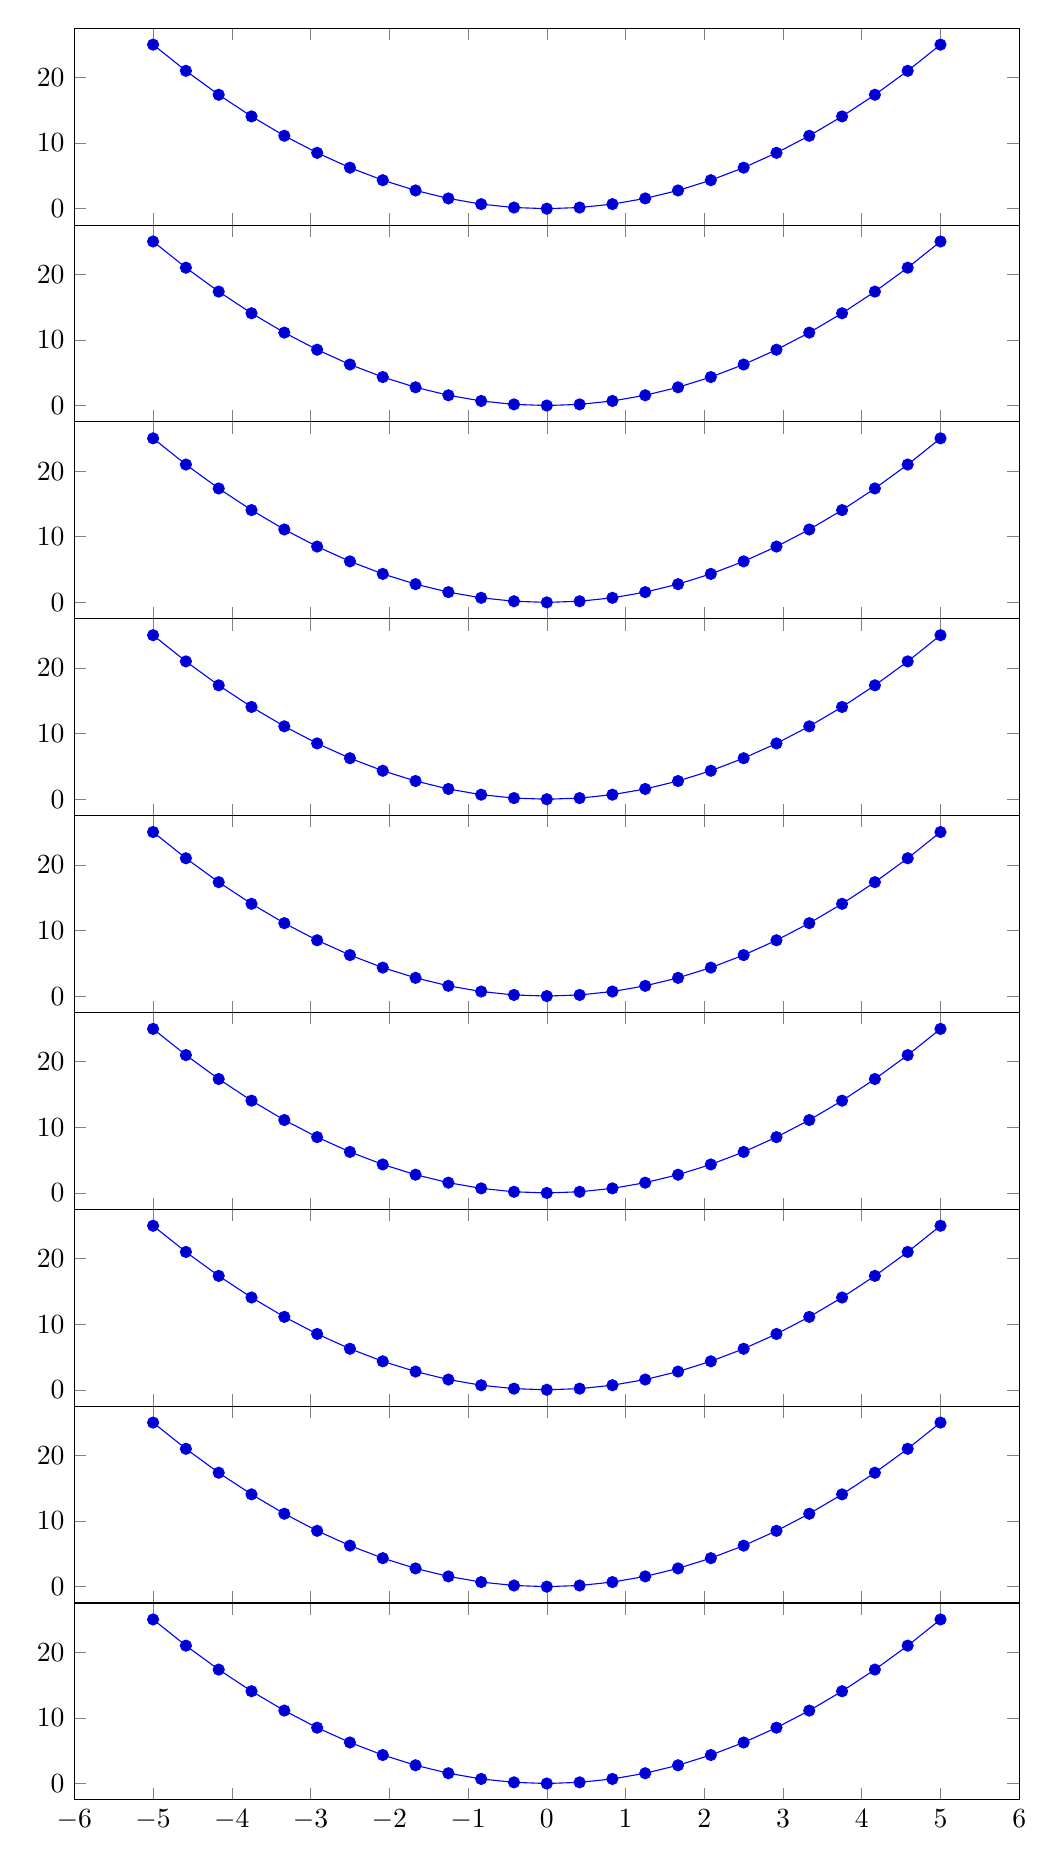
\begin{tikzpicture}
        \begin{groupplot}[
           group style={
              group name=geo1,
              group size=1 by 9,
              vertical sep=0pt,
              x descriptions at=edge bottom},
           width=12cm,
           height=2.5cm,
           scale only axis]
            \nextgroupplot
                \addplot {x^2};
            \nextgroupplot
                \addplot {x^2};
            \nextgroupplot
                \addplot {x^2};
            \nextgroupplot
                \addplot {x^2};
            \nextgroupplot
                \addplot {x^2};
            \nextgroupplot
                \addplot {x^2};
            \nextgroupplot
                \addplot {x^2}; 
            \nextgroupplot
                \addplot {x^2};
            \nextgroupplot
                \addplot {x^2};
        \end{groupplot}
    \end{tikzpicture}
\end{figure}
\subsection{A Graph}
\begin{figure}[H]
    \centering
    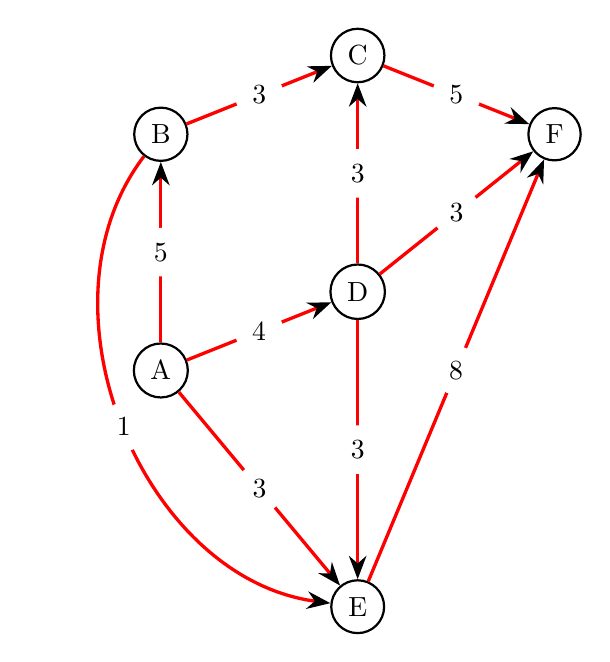
\begin{tikzpicture}
    \begin{scope}[every node/.style={circle,thick,draw}]
            \node (A) at (0,0) {A};
            \node (B) at (0,3) {B};
            \node (C) at (2.5,4) {C};
            \node (D) at (2.5,1) {D};
            \node (E) at (2.5,-3) {E};
            \node (F) at (5,3) {F};
        \end{scope}
        \begin{scope}[>={Stealth[black]},
                      every node/.style={fill=white,circle},
                      every edge/.style={draw=red,very thick}]
            \path [->] (A) edge node {$5$} (B);
            \path [->] (B) edge node {$3$} (C);
            \path [->] (A) edge node {$4$} (D);
            \path [->] (D) edge node {$3$} (C);
            \path [->] (A) edge node {$3$} (E);
            \path [->] (D) edge node {$3$} (E);
            \path [->] (D) edge node {$3$} (F);
            \path [->] (C) edge node {$5$} (F);
            \path [->] (E) edge node {$8$} (F); 
            \path [->] (B) edge[bend right=60] node {$1$} (E); 
        \end{scope}
    \end{tikzpicture}
    \caption{A Cool Graph from Graph Theory}
    \label{fig:graph_theory}
\end{figure}
Isn't Figure \ref{fig:graph_theory} awesome? It shows a graph.
\subsection{Awesome Spheres}
\begin{figure}[H]
    \centering
    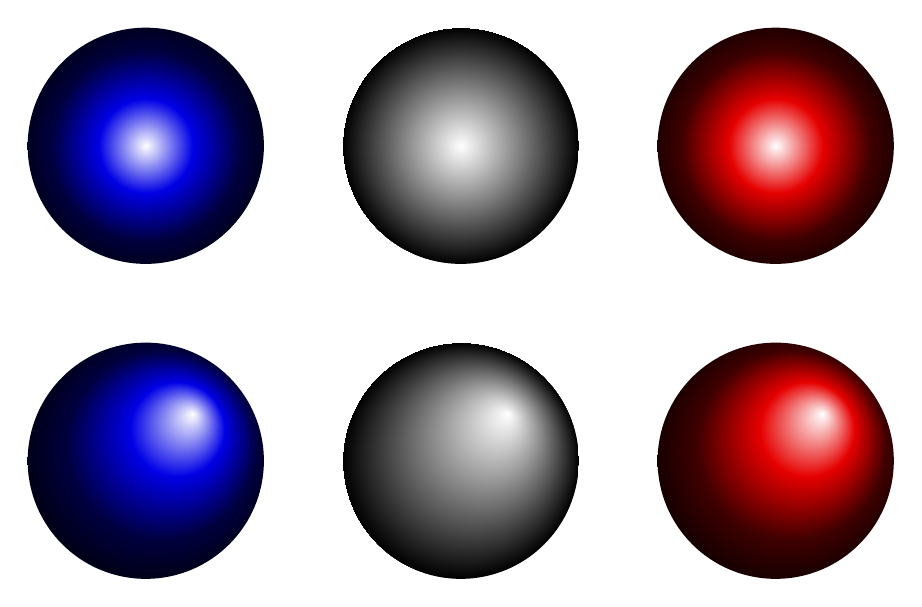
\begin{tikzpicture}
        \shade [shading=blue normal] (-5, 3.5) circle (1.5cm);
        \shade [shading=red normal] (3, 3.5) circle (1.5cm);
        \shade [shading=gray normal] (-1, 3.5) circle (1.5cm);
        \shade [shading=gray distorted] (-1, -0.5) circle (1.5cm);
        \shade [shading=blue distorted] (-5, -0.5) circle (1.5cm);
        \shade [shading=red distorted] (3, -0.5) circle (1.5cm);
    \end{tikzpicture}
    \caption{Spheres!}
    \label{fig:spheres}
\end{figure}
Figure \ref{fig:spheres} is also cool, but Jolene is cooler.
\subsection{Plotting Functions}
\begin{figure}[H]
    \centering
    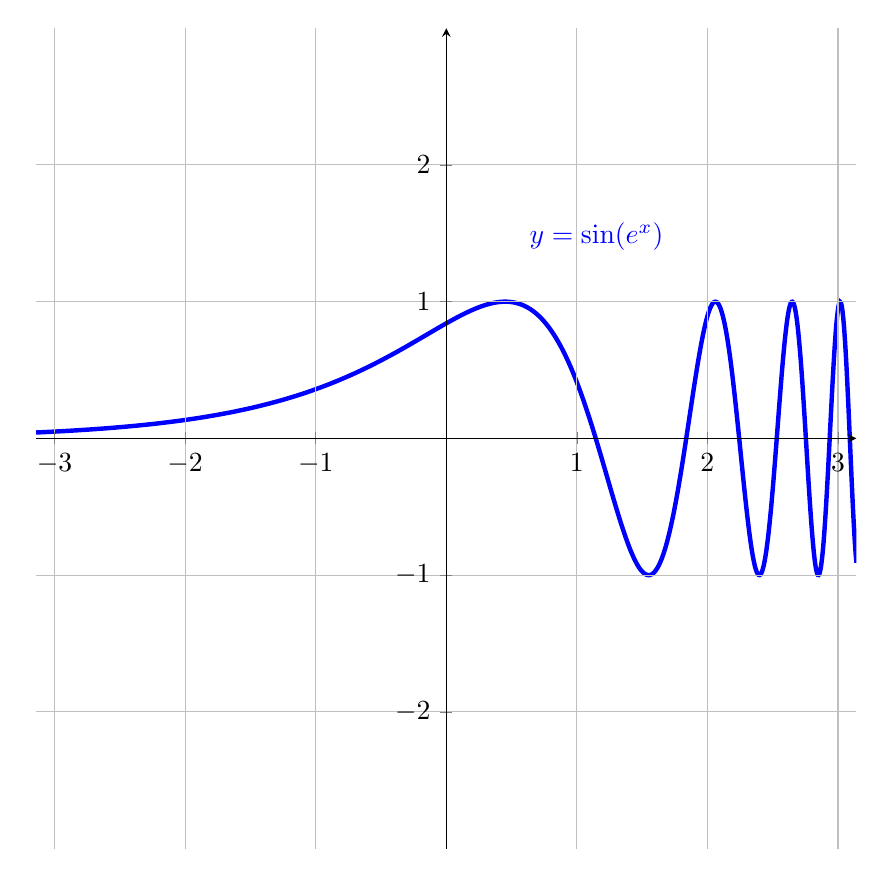
\begin{tikzpicture}
        \begin{axis}[
                axis y line=center,
                axis x line=middle, 
                axis on top=true,
                xmin=-pi,
                xmax=pi,
                ymin=-3,
                ymax=3,
                height=12.0cm,
                width=12.0cm,
                grid,
                xtick={-5,...,5},
                ytick={-2,-1,...,2},
                restrict y to domain=-3:3
            ]
            \addplot [domain=-pi:pi, samples=1000, mark=none, ultra thick, blue]
                {sin(deg(e^(x)))};
            \node [above, blue] at (axis cs: 1.15,1.3) {$y=\sin(e^{x})$};
        \end{axis}
    \end{tikzpicture}
    \caption{A Whacky Function!}
    \label{fig:whacky_function}
\end{figure}
\subsection{Awesome Tikz Examples}
\begin{figure}[H]
    \centering
    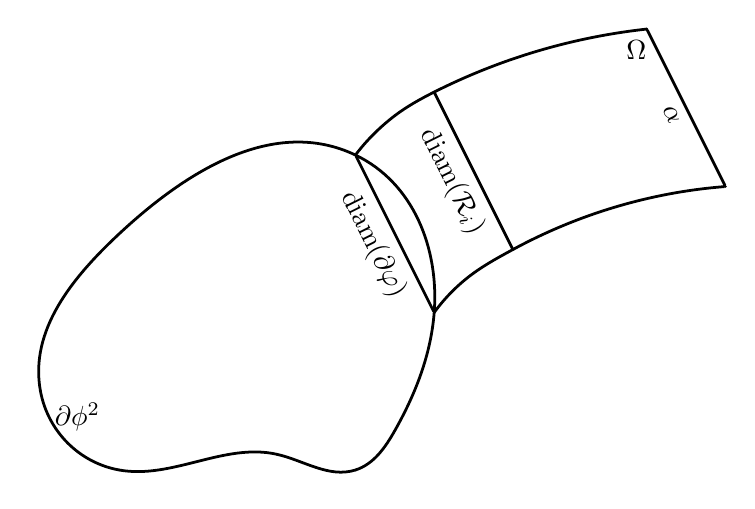
\begin{tikzpicture}[line width=1pt,line cap = round]
        \node[%
            fill=black, circle, inner sep=0pt, outer sep=0pt,
            label={[xshift=1pt]below right:$\partial \phi^2$}%
        ] at (0,1) (a) {};
        \node[fill=black, circle, inner sep=0pt, outer sep=0pt] at (1,3) (b) {};
        \node[fill=black, circle, inner sep=0pt, outer sep=0pt] at (4,4) (c) {};
        \node[fill=black, circle, inner sep=0pt, outer sep=0pt] at (5,2) (d) {};
        \node[fill=black, circle, inner sep=0pt, outer sep=0pt] at (4.5,.5) (e) {};
        \node[fill=black, circle, inner sep=0pt, outer sep=0pt] at (4,0) (f) {};
        \node[fill=black, circle, inner sep=0pt, outer sep=0pt] at (3,.2) (g) {};
        \node[fill=black, circle, inner sep=0pt, outer sep=0pt] at (1,0) (h) {};
        
        \path[draw,use Hobby shortcut,closed=true]
        (a) .. (b) .. (c) .. (d) .. (e) .. (f) .. (g) .. (h);
        
        \node[fill=black,circle,inner sep=0pt,outer sep=0pt] at (4.5,4.5) (i) {};
        \node[fill=black,circle,inner sep=0pt,outer sep=0pt] at (5,4.8) (j) {};
        \node[fill=black,circle,inner sep=0pt,outer sep=0pt,label={[xshift=4pt]below left:$\Omega$}] at (7.7,5.6) (k) {} ;
        \node[fill=black,circle,inner sep=0pt,outer sep=0pt,xshift=1cm,yshift=-2cm] at (4.5,4.5) (l) {};
        \node[fill=black,circle,inner sep=0pt,outer sep=0pt,xshift=1cm,yshift=-2cm] at (5,4.8) (m) {};
        \node[fill=black,circle,inner sep=0pt,outer sep=0pt,xshift=1cm,yshift=-2cm] at (7.7,5.6) (n) {};
        
        \draw (c) to [quick curve through={(i) . . (j)}] (k)
              (k) -- node[midway,below,sloped]{$\alpha$} (n)
              (n) to [quick curve through={(m) . . (l)}] (d)
              (m) -- node[midway,below,sloped]{$\operatorname{diam} (\mathcal{R}_i)$} (j)
              (d) -- node[midway,below,sloped]{$\operatorname{diam} (\partial \varphi)$} (c);
    \end{tikzpicture}
    \caption{Strange Geometry Thing!}
    \label{fig:Topology_Thing}
\end{figure}
\begin{figure}[H]
    \centering
    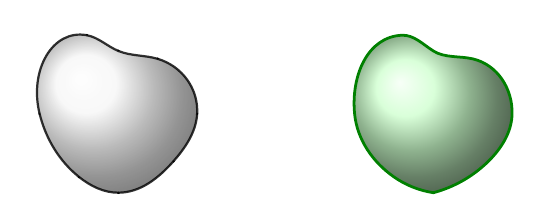
\begin{tikzpicture}[line width=1pt,line cap = round,>={Stealth[black]},every edge/.style={draw=black,very thick}]
        \node[fill=black,circle,inner sep=0pt,outer sep=0pt] at (-4,0) (a) {};
        \node[fill=black,circle,inner sep=0pt,outer sep=0pt] at (-4.5,0.2) (b) {};
        \node[fill=black,circle,inner sep=0pt,outer sep=0pt] at (-5,1) (c) {};
        \node[fill=black,circle,inner sep=0pt,outer sep=0pt] at (-4.4,2) (d) {};
        \node[fill=black,circle,inner sep=0pt,outer sep=0pt] at (-4, 1.8) (e) {};
        \node[fill=black,circle,inner sep=0pt,outer sep=0pt] at (-3.5, 1.7) (f) {};
        \node[fill=black,circle,inner sep=0pt,outer sep=0pt] at (-3,1) (g) {};
        \node[fill=black,circle,inner sep=0pt,outer sep=0pt] at (-3.3,0.4) (h) {};
        \node at (0,1) (i) {$X$};
                
        \path[draw,thick,use Hobby shortcut,closed=true,ball color=gray!10!white,opacity=0.8](a) .. (b) .. (c) .. (d) .. (e) .. (f) .. (g) .. (h);
        
        \filldraw[ball color=green!20!white, draw=green!50!black](0,0) to [quick curve through={(-0.5,0.2) .. (-1,1) .. (-0.4,2) .. (0, 1.8) .. (0.5, 1.7) .. (1,1) .. (0.7,0.4)}]  cycle;
    \end{tikzpicture}
    \caption{Blobs!}
    \label{fig:Blobs}
\end{figure}
\end{document}